%% ==========================================================================
%%  Tema Beamer institucional: Mesoamérica Malaria (IREM) · BID
%%
%%  Réplica de ppt_resultados_IREM_2025_master_logos.pptx, que es el master
%%  vigente. Ese archivo trae su propia guía de estilo en la lámina 2:
%%  tipografía, paleta y escala de puntos declaradas por la institución.
%%
%%  OJO con lo que el archivo declara y no cumple: el fontScheme del tema
%%  dice Arial y los layouts arrastran restos del export de Google Slides
%%  (título de 40 pt en #0070C0). Nada de eso es la identidad. La identidad
%%  es la lámina 2 más lo que aplican de hecho las láminas de contenido.
%%
%%  Conversión del lienzo de PowerPoint (338.667 x 190.5 mm) al de Beamer
%%  (160 x 90 mm): factor 0.472441. Toda medida que aparezca comentada como
%%  "PPT" está en el lienzo original; la que va en el código, ya convertida.
%%
%%  Densidad: se respeta la geometría del master, pero no su escala de
%%  cuerpo. El master pide 14-16 pt sobre un lienzo del doble de ancho, que
%%  convertidos son 6.6-7.6 pt: ilegible proyectado. El cuerpo va en 10 pt.
%%  Los elementos de despliegue (portada, portadilla, cierre, numerales) sí
%%  usan el valor convertido del master, porque ahí sí funciona.
%% ==========================================================================

\usepackage{fontspec}
\usepackage{xcolor}
\usepackage{graphicx}
\usepackage{tikz}
\usepackage{tcolorbox}
\usepackage{colortbl}
%% `array` da las columnas m{...}, que centran la celda verticalmente. Sin
%% ellas, en una tabla con una columna de texto ancha y varias de cifras, el
%% encabezado de la ancha se descuelga respecto de los otros.
\usepackage{array}

%% --- Paleta institucional --------------------------------------------------
%%  Medida de las figuras del master y confirmada contra su lámina 2.
\definecolor{iremazul}{HTML}{367CBC}    % títulos, portadillas, cabecera de tabla
\definecolor{iremverde}{HTML}{98CE63}   % numerales, cajas, viñetas
\definecolor{grisoscuro}{HTML}{404040}  % texto principal
\definecolor{grisclaro}{HTML}{9B9B9D}   % texto secundario, notas al pie
\definecolor{grissuave}{HTML}{EFEEEE}   % fondos y texto sobre azul
%%  La barra de la portada no usa el verde institucional sino este otro, un
%%  punto más apagado. Es lo que trae el master; no lo unifiques.
\definecolor{verdeportada}{HTML}{92C14B}
%%  Escala de calor de tablas, tal como la declara la lámina 16 del master.
\definecolor{calorbajo}{HTML}{F8696B}
\definecolor{calormedio}{HTML}{FFEB84}
\definecolor{caloralto}{HTML}{63BE7B}

%% --- Rutas de los logotipos ------------------------------------------------
\graphicspath{{_extensions/irem/logos/}{logos/}{./}}

%% --- Tipografía ------------------------------------------------------------
%%  Montserrat, que es la que el master trae embebida en sus cuatro variantes.
%%  No está en macOS: viene del paquete `montserrat` de TeX Live, así que
%%  fontspec la busca por nombre de archivo vía kpathsea. Si falta el paquete
%%  (`tlmgr install montserrat`) se cae a Arial, que es lo que el fontScheme
%%  del master declara y lo que usan de hecho las plantillas viejas de IREM.
\IfFontExistsTF{Montserrat-Regular.otf}{%
  \setsansfont{Montserrat}[
    Scale          = 1,
    Extension      = .otf,
    UprightFont    = *-Regular,
    BoldFont       = *-Bold,
    ItalicFont     = *-Italic,
    BoldItalicFont = *-BoldItalic]%
}{%
  \IfFontExistsTF{Montserrat}{\setsansfont{Montserrat}[Scale=1]}{%
    \IfFontExistsTF{Arial}{\setsansfont{Arial}[Scale=1]}{\setsansfont{Helvetica Neue}[Scale=1]}}%
}
\IfFontExistsTF{Menlo}{\setmonofont{Menlo}[Scale=0.8]}{\setmonofont{Courier New}[Scale=0.88]}
\renewcommand{\familydefault}{\sfdefault}
\usefonttheme{professionalfonts}

%% --- Colores de Beamer -----------------------------------------------------
\setbeamercolor{normal text}{fg=grisoscuro, bg=white}
\setbeamercolor{structure}{fg=iremverde}
%%  Sin fondo: si la caja del título lleva bg=white, pinta una banda blanca de
%%  ancho completo sobre el fondo y borra el degradado gris en la parte de
%%  arriba de cada lámina. Se nota al poner una lámina junto a otra del master.
\setbeamercolor{frametitle}{fg=iremazul, bg=}
\setbeamercolor{title}{fg=grisoscuro}
\setbeamercolor{subtitle}{fg=grisoscuro}
\setbeamercolor{itemize item}{fg=iremverde}
\setbeamercolor{itemize subitem}{fg=iremazul}
\setbeamercolor{enumerate item}{fg=iremazul}
\setbeamercolor{alerted text}{fg=iremazul}
\setbeamercolor{block title}{fg=white, bg=iremazul}
\setbeamercolor{block body}{fg=grisoscuro, bg=grissuave}

%% --- Escala tipográfica ----------------------------------------------------
%%  Columna «master» = punto declarado en su lámina 2, ya convertido a Beamer.
%%                            master   aquí
%%  título de lámina           15.1     16
%%  subtítulo                   9.4     10.5
%%  cuerpo y punteos          6.6-7.6   10
%%  tabla                       6.6     8.5
%%  nota al pie                 5.0     7
\setbeamerfont{frametitle}{size=\fontsize{16}{20}\selectfont, series=\bfseries}
\setbeamerfont{normal text}{size=\fontsize{10}{14.5}\selectfont}
\setbeamerfont{itemize/enumerate body}{size=\fontsize{10}{15}\selectfont}
\setbeamerfont{itemize/enumerate subbody}{size=\fontsize{8.5}{13}\selectfont}
\setbeamerfont{footline}{size=\fontsize{7}{9}\selectfont}

%% --- Márgenes --------------------------------------------------------------
%%  El cuerpo se alinea con el título, y los dos van a 12.5 mm.
%%
%%  Ojo con este número: el placeholder del master está en x=23.7 mm, que
%%  convertido daría 11.2, pero el TEXTO no arranca ahí. PowerPoint mete un
%%  margen interno de 0.1 in en toda caja de texto, así que lo que se ve
%%  empieza en 26.5 mm PPT → 12.5 mm. Medido en el PDF del master en las
%%  láminas 3, 11, 12, 13 y 17: siempre 26.4 a 26.5. Si tomas la coordenada
%%  del XML sin sumarle ese margen, toda la lámina queda 1.3 mm corrida.
\setbeamersize{text margin left=12.2mm, text margin right=12.2mm}
\setlength{\parskip}{0.5em}

%%  El entorno `columns` de beamer ignora esos márgenes: sin `onlytextwidth`
%%  se extiende sobre casi todo el ancho del papel y una lámina de dos
%%  columnas arranca 3.6 mm a la izquierda del título, que se nota enseguida
%%  al ponerla junto a cualquier otra. Quarto genera `\begin{columns}[T]` sin
%%  opciones, así que la opción se inyecta aquí, de una vez para todas.
\let\iremColumns\columns
\let\iremEndColumns\endcolumns
\renewenvironment{columns}[1][]{\iremColumns[#1,onlytextwidth]}{\iremEndColumns}

\setbeamertemplate{navigation symbols}{}

%% --- Listas ----------------------------------------------------------------
%%  OJO, esto sorprende: en este master el PRIMER nivel no lleva viñeta. El
%%  layout «Titulo y contenido» declara <a:buNone/> en lvl1 y reserva solo una
%%  sangría (marL 457200 EMU = 12.7 mm PPT → 6.0 mm). El punto aparece recién
%%  en el segundo nivel, y en gris oscuro, no en verde.
%%
%%  Lo que separa un punto del siguiente es el aire, no el glifo: el master
%%  pone spcBef de 10 pt (→ 4.7). Si le quitas ese aire, la lámina se lee como
%%  un párrafo partido en trozos y la decisión de no usar viñeta se vuelve un
%%  error de composición.
\setbeamertemplate{itemize item}{}
\setbeamertemplate{itemize subitem}{\color{grisoscuro}\scriptsize\raisebox{0.15ex}{\textbullet}}
%%  Sin sangría en el primer nivel: en el PDF del master el cuerpo arranca en
%%  la misma x que el título (26.4 contra 26.5 mm), no 6 mm más adentro. El
%%  layout declara marL=457200, pero eso no es lo que se compone; manda el
%%  render. El segundo nivel sí entra, y ahí aparece el punto.
\setlength{\leftmargini}{0mm}
\setlength{\leftmarginii}{6.0mm}

%%  Pero `enumerate` sí necesita sitio: con leftmargini en cero, el número
%%  cuelga hacia la izquierda y se sale del margen de la lámina. Se le da su
%%  propio margen justo antes de que el entorno monte la lista, que es el
%%  único momento en que \leftmargini todavía se lee.
\AtBeginEnvironment{enumerate}{\setlength{\leftmargini}{5mm}}
\AtBeginEnvironment{itemize}{\setlength{\leftmargini}{0mm}}

%%  El aire entre puntos hay que meterlo parcheando \itemize, no por plantilla.
%%  Comprobado midiendo el PNG: con
%%  \setbeamertemplate{itemize/enumerate body begin}{\setlength{\itemsep}{...}}
%%  la separación no cambia ni un píxel, porque beamer fija \itemsep después de
%%  componer esa plantilla. Con \apptocmd el \setlength cae ya dentro de la
%%  lista y sí manda. Si algún día parece que no se aplica, mide antes de tocar.
%%
%%  El valor sale de la proporción del master: spcBef 10 pt sobre cuerpo de
%%  18 pt, o sea 0.556 del tamaño de letra; con cuerpo de 10 pt son 5.5.
\usepackage{etoolbox}
\apptocmd{\itemize}{\setlength{\itemsep}{5.5pt}}{}{}
\apptocmd{\enumerate}{\setlength{\itemsep}{5.5pt}}{}{}

%%  …y todavía falta un paso, porque el parche anterior por sí solo no se ve.
%%  Toda lista de Markdown sin renglón en blanco entre puntos la escribe pandoc
%%  con \tightlist, que es literalmente \itemsep=0pt \parskip=0pt, y como se
%%  ejecuta dentro de la lista pisa lo que puso \apptocmd. O sea: en un .qmd
%%  normal, TODAS las listas salen apretadas. Se redefine \tightlist para que
%%  conserve el aire del master.
%%
%%  Va en \AtBeginDocument porque \tightlist lo declara la plantilla de pandoc
%%  y no hay garantía de que ya exista cuando se lee este archivo.
\AtBeginDocument{%
  \providecommand{\tightlist}{}%
  \renewcommand{\tightlist}{\setlength{\itemsep}{5.5pt}\setlength{\parskip}{0pt}}%
}

%% --- Decoración fija de las láminas de contenido ---------------------------
%%  El master NO lleva chevron. Lo que lleva son los dos logotipos del pie, y
%%  van al revés que en las plantillas viejas de IREM:
%%
%%    mesoamérica MALARIA   PPT (4.23, 164.12) 44.38 mm de ancho  → izquierda
%%    BID                   PPT (310.87, 166.24) 20.85 mm         → derecha
%%
%%  El BID del pie va recortado: el master le quita el 29.878% superior, que
%%  es donde dice «Administrador». El asset ya viene recortado; no uses el
%%  logotipo completo aquí o aparecerá esa palabra suelta.
%%
%%  Todo va en el pie y no en la cabecera: el pie se compone DESPUÉS del
%%  título de lámina, así que nada de lo que se dibuje aquí queda por debajo.
%%  --- Fondo de lámina ------------------------------------------------------
%%  El fondo del master: blanco con un degradado gris muy tenue en las
%%  esquinas y, al pie, la franja azul sobre verde a sangre.
%%
%%  Va como imagen y no dibujado a mano porque en el master TAMPOCO es una
%%  forma: es el relleno de fondo del slide master (`<p:bg>` con un blipFill),
%%  que es justo el sitio donde no lo busca uno. Se buscó primero entre las
%%  formas de las láminas y de los layouts, y ahí no está; de ahí salió la
%%  conclusión equivocada de que el .pptx no la traía. Sí la trae.
%%
%%  Usar la imagen entera en vez de dos rectángulos tiene dos ventajas: sale
%%  el degradado, que a mano no estaba, y la franja queda exacta sin depender
%%  de dos longitudes calibradas. Medida en el asset: azul de 86.04 a 88.30 mm
%%  y verde de 88.30 al borde.
%%
%%  Pesa 23 KB porque es casi todo blanco.
\setbeamertemplate{background canvas}{%
  
\includegraphics[width=\paperwidth, height=\paperheight]{fondo.png}%
}

\newcommand{\iremLogosNodos}{%
  \node[anchor=north west, inner sep=0pt]
    at ([shift={(2.0mm,-77.53mm)}]current page.north west)
    {
\includegraphics[width=20.97mm]{logo-mesoamerica.png}};
  \node[anchor=north west, inner sep=0pt]
    at ([shift={(146.87mm,-78.53mm)}]current page.north west)
    {
\includegraphics[width=9.85mm]{logo-bid.png}};%
}
%%  Comando público para las láminas `plain`, que no llevan pie.
\newcommand{\logosPie}{%
  \begin{tikzpicture}[remember picture, overlay]\iremLogosNodos\end{tikzpicture}%
}

\setbeamertemplate{headline}{}
\setbeamertemplate{footline}{%
  \ifnum\insertframenumber>1\relax
    \begin{tikzpicture}[remember picture, overlay]\iremLogosNodos\end{tikzpicture}%
  \fi
}
%% Sin numeración de láminas, por decisión de formato.
\setbeamertemplate{page number in head/foot}{}

%% --- Portada: réplica del layout TAPA --------------------------------------
%%  Piezas y posiciones (PPT → Beamer):
%%    logo mesoamérica   (16.27, 17.84)  75.05 ancho  → (7.69, 8.43)  35.46
%%    barra verde        (13.90, 50.16) 107.0 x 9.4   → (6.57, 23.70) 50.55 x 4.44
%%    volanta            centrada sobre la barra verde
%%    título            (13.90, 65.00) 155.5 ancho    → (6.57, 30.71) 73.46
%%    autoría/lugar      (16.27, 142.2) 83.5 ancho    → (7.69, 67.18) 39.45
%%    cintilla donantes  (15.03, 160.76) 140.34 ancho → (7.10, 75.95) 66.30
%%    fotografía        (193.08, -0.61) 145.88x182.89 → (91.21,-0.29) 68.92 x 86.40
%%
%%  A DIFERENCIA DEL MASTER ANTERIOR, la portada se compone de piezas sueltas:
%%  la fotografía es un JPG independiente, no una imagen que ya trae el panel
%%  del logotipo incrustado. Por eso aquí sí se posiciona elemento por
%%  elemento y no hay que temerle al recorte.
%%
%%  La foto ya viene recortada al srcRect del master (l=43.716%, r=3.112%),
%%  que se queda con la mitad derecha de la imagen original. No la recortes
%%  otra vez ni la sustituyas por la original completa: el encuadre cambia.
%%
%%  Y va en PNG, no en JPEG, aunque el master la traiga en JPEG y el JPEG
%%  pese cuatro veces menos. Razón: xelatex incrusta el JPEG perfectamente
%%  (queda un DCTDecode válido en el PDF) pero el poppler que usa
%%  pdftools::pdf_convert lo pinta en blanco. O sea que el PDF sale bien y la
%%  revisión por PNG lo muestra roto, que es la peor combinación posible:
%%  lleva a «arreglar» una portada que no estaba mal. Con PNG coinciden el
%%  PDF y la revisión. No la vuelvas a convertir a JPEG.
%%
%%  Sangra arriba y a la derecha, y se detiene a 3.88 mm del borde inferior.
%%  Esa franja blanca de abajo es del diseño, no un defecto: es el aire donde
%%  respira la cintilla de donantes. No la elimines.
%%
%%  En la portada las palabras no se parten. Con babel en español no basta
%%  \hyphenpenalty=10000, así que se anula el \hyphenchar de la fuente activa
%%  después de cada \selectfont. Si añades un elemento, repite ese
%%  \hyphenchar o volverás a ver cortes como "cuan-do".
\newsavebox{\iremCajaVolanta}
\setbeamertemplate{title page}{%
  %% La volanta se compone ANTES de abrir el tikzpicture. Dentro, TikZ agrupa
  %% cada elemento del path y la asignación del box se pierde: la barra sale
  %% pintada pero vacía, sin ningún error que lo delate.
  %% La volanta va en BLANCO sobre la barra, no en gris. El XML no lo dice
  %% (hereda, y la herencia acaba en negro), pero en el PDF del master los
  %% píxeles claros dentro de la barra son #ECEBE7. Manda el render.
  \sbox{\iremCajaVolanta}{%
    \bfseries\color{grissuave}\fontsize{7}{9}\selectfont\hyphenchar\font=-1\relax
    \insertsubtitle}%
  \begin{tikzpicture}[remember picture, overlay]
    \node[anchor=north west, inner sep=0pt]
      at ([shift={(91.21mm,0.29mm)}]current page.north west)
      {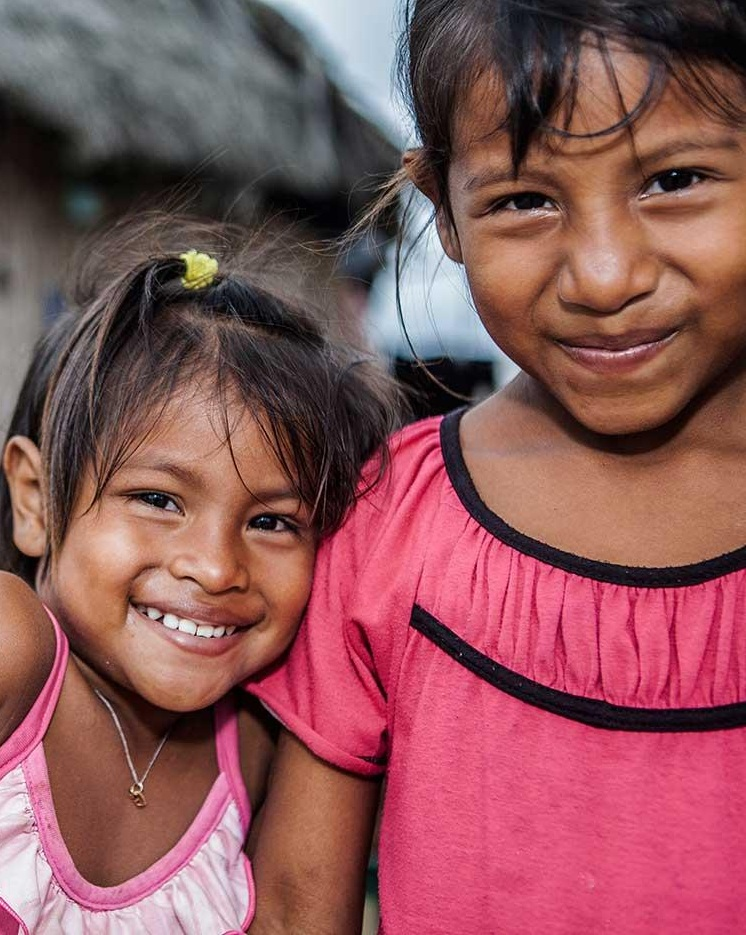
\includegraphics[height=86.40mm]{portada-foto.png}};
    \node[anchor=north west, inner sep=0pt]
      at ([shift={(7.69mm,-8.43mm)}]current page.north west)
      {
\includegraphics[width=35.46mm]{logo-mesoamerica.png}};
    %% Barra verde con la volanta encima. La volanta sale del `subtitle`:
    %% en el master ese renglón dice el evento y el mes, en versalitas.
    %% Esquinas redondeadas: medido en el PDF del master, el sangrado de la
    %% esquina cae de 1.40 mm PPT a cero, o sea 0.66 mm en Beamer. Es una
    %% curva discreta; a tamaño de pantalla parece más pronunciada de lo que
    %% es porque en la lámina 1 del master hay DOS barras superpuestas (una
    %% del layout y otra que el autor puso encima, desfasadas 4.2 mm). La
    %% buena es la del layout, que es la que está aquí.
    \fill[verdeportada, rounded corners=0.66mm]
      ([shift={(6.57mm,-23.70mm)}]current page.north west) rectangle
      ([shift={(57.12mm,-28.14mm)}]current page.north west);
    \ifx\insertsubtitle\empty\else
      %% La volanta va en UNA línea dentro de la barra, y la barra mide lo que
      %% mide. Como el texto lo escribe quien haga la presentación y puede ser
      %% largo, la caja ya compuesta se mide y solo si se pasa de los 47 mm
      %% útiles se encoge. Con `text width` se envolvería a dos renglones y el
      %% segundo caería fuera de la barra verde.
      \node[anchor=center, inner sep=0pt]
        at ([shift={(31.84mm,-25.92mm)}]current page.north west)
        {\ifdim\wd\iremCajaVolanta>47mm
           \resizebox{47mm}{!}{\usebox{\iremCajaVolanta}}%
         \else
           \usebox{\iremCajaVolanta}%
         \fi};
    \fi
    \node[anchor=north west, text width=73.46mm, align=left, inner sep=0pt]
      at ([shift={(6.57mm,-30.71mm)}]current page.north west)
      {\bfseries\color{grisoscuro}\fontsize{20}{25}\selectfont\hyphenchar\font=-1\relax
       \inserttitle};
    %% Autoría y fecha ocupan el renglón gris que en el master lleva el país.
    \node[anchor=north west, text width=60mm, align=left, inner sep=0pt]
      at ([shift={(7.69mm,-67.18mm)}]current page.north west)
      {\color{grisclaro}\fontsize{9}{12}\selectfont\hyphenchar\font=-1\relax
       \insertauthor
       \ifx\insertdate\empty\else
         \\[0.8mm]{\fontsize{8}{11}\selectfont\hyphenchar\font=-1\relax\insertdate}%
       \fi};
    \node[anchor=north west, inner sep=0pt]
      at ([shift={(7.10mm,-75.95mm)}]current page.north west)
      {
\includegraphics[width=66.30mm]{cintilla-donantes.png}};
    %% La portada también lleva franja: en el PDF del master está en las 20
    %% láminas sin excepción. El pie no se compone en la lámina 1, así que
    %% aquí se dibuja a mano.
  \end{tikzpicture}%
}

%% --- Título de lámina ------------------------------------------------------
%%  PPT (23.7, 11.0) 291.3 x 15.3 → (11.2, 5.20) 137.6 x 7.23.
%%  Los dos \vspace están calibrados contra el PDF del master, no a ojo. La
%%  referencia es el tope de las mayúsculas del título, que es lo único
%%  estable: el centro de la caja cambia según qué letras lleve el título.
%%  En el master ese tope cae en 12.8 mm PPT → 6.05 mm, y el primer renglón
%%  del cuerpo entre 23.5 y 25.2. Si tocas uno, vuelve a medir los dos.
\setbeamertemplate{frametitle}{%
  \vspace*{2.78mm}%
  \begin{beamercolorbox}[wd=\paperwidth, leftskip=12.2mm, rightskip=12.2mm]{frametitle}%
    \usebeamerfont{frametitle}\insertframetitle\par%
  \end{beamercolorbox}%
  \vspace{6.85mm}%
}

%% --- Portadilla de sección -------------------------------------------------
%%  NO es azul a sangre. En el master vigente la portadilla es blanca, con el
%%  título centrado en azul y los mismos logotipos del pie que el resto.
%%  PPT (52.3, 73.71) 234.02 x 43.13 → (24.71, 34.82) 110.56 x 20.38,
%%  44 pt bold → 20.8; se usan 21.
\newcommand{\laminaPortadilla}[1]{%
  \begingroup
  \setbeamertemplate{headline}{}
  \setbeamertemplate{footline}{}
  \begin{frame}[plain, noframenumbering]
    \begin{tikzpicture}[remember picture, overlay]
      \node[anchor=north, text width=110.56mm, align=center, inner sep=0pt]
        at ([shift={(80mm,-34.82mm)}]current page.north west)
        {\bfseries\color{iremazul}\fontsize{21}{26}\selectfont #1};
      \iremLogosNodos
    \end{tikzpicture}%
  \end{frame}
  \endgroup
}
\AtBeginSection[]{\laminaPortadilla{\insertsectionhead}}

%% --- Numerales 01 / 02 / 03 ------------------------------------------------
%%  El elemento de firma del master: una columna de cifras verdes enormes,
%%  cada una junto a una caja verde con su punto. Aparece en tres layouts.
%%
%%    cifra  PPT (22.3, 56.6) 26.0 ancho, 44 pt → (10.53, 26.74) 12.28, 21 pt
%%    caja   PPT (48.4, 48.0) 152.7 x 33.1      → (22.87, 22.68) 72.14 x 15.64
%%    paso entre filas  PPT 36.4 → 17.20 mm  (caja 15.64 + 1.56 de aire)
%%
%%  Máximo tres por lámina: el master nunca pone una cuarta y no cabe.
%%  Las filas van en posición ABSOLUTA, no apiladas en el flujo del texto.
%%  Apilándolas con \par y \vspace, el \parskip y el interlineado se suman a
%%  cada paso: medido, el paso salía en 21.7 mm en vez de 17.20 y la tercera
%%  caja terminaba encima del logotipo del pie. Con la posición calculada
%%  desde el contador, la fila n cae siempre donde el master la pone.
%%
%%  Por eso hay entorno: `numerados` es lo que pone el contador en cero al
%%  empezar cada lámina. Sin él, la segunda lámina con numerales arrancaría
%%  en la fila 4, o sea fuera de la lámina.
\newcounter{iremNum}
\newenvironment{numerados}{\setcounter{iremNum}{0}}{}
\newcommand{\numerado}[2]{%
  \stepcounter{iremNum}%
  \begin{tikzpicture}[remember picture, overlay]
    %% fila n: caja en y = 22.68 + (n-1) * 17.20 ; cifra centrada en esa caja
    \pgfmathsetmacro{\iremYcaja}{22.68 + (\value{iremNum}-1)*17.20}
    \pgfmathsetmacro{\iremYeje}{\iremYcaja + 7.82}
    \node[anchor=west, inner sep=0pt]
      at ([shift={(10.53mm,-\iremYeje mm)}]current page.north west)
      {\fontsize{21}{23}\selectfont\bfseries\color{iremverde}#1};
    \node[anchor=west, inner sep=0pt]
      at ([shift={(22.87mm,-\iremYeje mm)}]current page.north west)
      {\begin{tcolorbox}[nobeforeafter,
         width=72.14mm, height=15.64mm, valign=center,
         colback=iremverde, colframe=iremverde,
         boxrule=0pt, arc=0.6mm,
         left=3mm, right=3mm, top=1.5mm, bottom=1.5mm]
         %% Sin partir palabras: en una caja de 72 mm un corte se lee como error.
         \raggedright\hyphenpenalty=10000\exhyphenpenalty=10000\relax
         {\fontsize{9}{11.5}\selectfont\color{grisoscuro}#2\par}
       \end{tcolorbox}};
  \end{tikzpicture}%
}

%% --- Caja de realce a la derecha -------------------------------------------
%%  El recuadro azul de contorno del layout «2_Titulo y contenido»: acompaña a
%%  los numerales con la advertencia o el matiz que no cabe en ellos.
%%  PPT (239.2, 73.0) 77.2 x 47.7 → (113.01, 34.49) 36.47 x 22.54, 18 pt → 8.5.
\newcommand{\realce}[1]{%
  \begin{tikzpicture}[remember picture, overlay]
    \node[anchor=north west, draw=iremazul, line width=0.35mm, rounded corners=0.6mm,
          text width=32.5mm, align=center, inner sep=2mm, minimum height=22.54mm]
      at ([shift={(113.01mm,-34.49mm)}]current page.north west)
      {\color{iremazul}\fontsize{9}{12}\selectfont #1};
  \end{tikzpicture}%
}

%% --- Panel lateral derecho -------------------------------------------------
%%  La columna de texto que el layout «1_Titulo y contenido» pone a la derecha
%%  de los numerales. PPT (219.1, 49.1) 102.5 ancho → (103.51, 23.20) 48.42.
\newcommand{\panelDerecho}[1]{%
  \begin{tikzpicture}[remember picture, overlay]
    \node[anchor=north west, text width=48.42mm, align=left, inner sep=0pt]
      at ([shift={(103.51mm,-23.20mm)}]current page.north west)
      {\color{grisoscuro}\fontsize{9}{12.5}\selectfont #1};
  \end{tikzpicture}%
}

%% --- Cierre ----------------------------------------------------------------
%%  Layout «Cierre»: el saludo grande, la banda con los dos logotipos y la
%%  bajada. No lleva los logotipos del pie, porque la banda ya los trae.
%%    saludo  PPT (23.34, 37.72) 292.10 ancho, 54 pt → (11.03, 17.82) 138.0, 26
%%    banda   PPT (36.19, 80.29) 267.62 x 58.69      → (17.10, 37.93) 126.42
%%    bajada  PPT (84.72, 167.08) 171.20 ancho, 12pt → (40.02, 78.93) 80.88, 8
%%
%%  Va dentro de una lámina `## {.plain}`. No crea su propio frame: Quarto ya
%%  tiene la lámina abierta.
\newcommand{\laminaGracias}[1][¡Muchas gracias!]{%
  \begin{tikzpicture}[remember picture, overlay]
    \node[anchor=north, text width=138mm, align=center, inner sep=0pt]
      at ([shift={(80mm,-17.82mm)}]current page.north west)
      {\bfseries\color{iremazul}\fontsize{26}{32}\selectfont #1};
    \node[anchor=north west, inner sep=0pt]
      at ([shift={(17.10mm,-37.93mm)}]current page.north west)
      {
\includegraphics[width=126.42mm]{cierre-logos.png}};
    \node[anchor=north, text width=100mm, align=center, inner sep=0pt]
      at ([shift={(80mm,-78.93mm)}]current page.north west)
      {\color{grisoscuro}\fontsize{8}{11}\selectfont
       Iniciativa Regional para la Eliminación de la Malaria};
    %% El cierre es `plain` y no pasa por el pie, así que la franja se dibuja
    %% aquí a mano. Sin esto es la única lámina del deck que se queda sin ella.
  \end{tikzpicture}%
}

%% --- Lámina de una sola idea -----------------------------------------------
\newcommand{\ideaGrande}[1]{%
  \vspace*{\fill}
  \begin{center}
    {\fontsize{20}{26}\selectfont\bfseries\color{iremazul} #1\par}
  \end{center}
  \vspace*{\fill}
}

%% --- Cifra destacada -------------------------------------------------------
\newcommand{\cifra}[2]{%
  \vspace*{\fill}
  \begin{center}
    {\fontsize{44}{48}\selectfont\bfseries\color{iremverde} #1\par}
    \vskip0.35em
    {\fontsize{12}{16}\selectfont\color{grisclaro} #2\par}
  \end{center}
  \vspace*{\fill}
}

%% --- Momento participativo -------------------------------------------------
\newcommand{\pregunta}[1]{%
  \vspace*{\fill}
  \begin{center}
    {\fontsize{9}{11}\selectfont\bfseries\color{iremverde} PREGUNTA AL EQUIPO\par}
    \vskip0.7em
    {\fontsize{18}{23}\selectfont\bfseries\color{grisoscuro} #1\par}
  \end{center}
  \vspace*{\fill}
}

%% --- Caja de concepto ------------------------------------------------------
%%  \concepto{término}{en una frase}
%%
%%  No sale del master, pero se queda: para láminas de vocabulario una rejilla
%%  de cajas delimita cada término, que es justo lo que una lista no hace.
%%  Reestilizada al master: filete verde, fondo gris suave, título en azul.
%%
%%  Dos por fila separadas con \hfill: 2 x 66 mm caben en los 137.6 mm de
%%  ancho de texto. Para tres conceptos, dos filas (2 + 1), no tres cajas
%%  angostas, para que el ancho no cambie entre láminas.
\newcommand{\concepto}[2]{%
  \begin{tcolorbox}[nobeforeafter, box align=top,
    width=66mm, height=20mm, valign=top,
    colback=grissuave, colframe=iremverde,
    boxrule=0pt, leftrule=1.4mm, arc=0.8mm,
    left=3mm, right=2.5mm, top=2mm, bottom=1mm]
    \raggedright\hyphenpenalty=10000\exhyphenpenalty=10000\relax
    {\fontsize{11}{13}\selectfont\bfseries\color{iremazul}#1\par}
    \vspace{1.2mm}
    {\fontsize{8.5}{11}\selectfont\color{grisoscuro}#2\par}
  \end{tcolorbox}%
}

%% --- Nota al pie de lámina -------------------------------------------------
%%  El master remata sus láminas de tabla y de gráfico con una nota en gris
%%  de 10.5 pt (→ 5, aquí 7). Es donde van los denominadores y las salvedades.
%%  El \vspace del final no es decorativo: en una lámina donde la nota va
%%  después de un \vspace*{\fill} (\cifra, \ideaGrande, \pregunta), el relleno
%%  la empuja hasta el borde del área de texto de beamer, que baja más que los
%%  77 mm útiles, y la nota termina encima del logotipo del pie. Con estos 4 mm
%%  el relleno cede y la nota se queda arriba. En una lámina normal, donde la
%%  nota sigue a una tabla, no se nota: son 4 mm de aire al final de todo.
\newcommand{\notaPie}[1]{%
  \par\vspace{1.5mm}
  {\fontsize{7}{9}\selectfont\color{grisclaro}#1\par}
  \vspace{4mm}
}

%% --- Tablas ----------------------------------------------------------------
%%  El master trae cuatro layouts de tabla, así que la tabla es un ciudadano
%%  de primera aquí. Estilo: cabecera azul con texto gris suave en negrita y
%%  versalitas, cuerpo sin relleno en gris oscuro, sin filete vertical.
%%
%%  Hay dos caminos, y conviene saber cuál se está tomando.
%%
%%  1. Tabla de Markdown. Sale con la tipografía y los filetes institucionales
%%     (gris, finos) pero SIN la banda azul de cabecera. Sirve para tablas
%%     pequeñas y de paso.
%%
%%  2. Entorno `tablaIrem`. Es la tabla del master: banda azul, texto gris
%%     suave en negrita, cuerpo en gris oscuro. Úsalo cuando la tabla sea el
%%     contenido de la lámina, que en este master es casi siempre.
%%
%%  No se intenta parchear el \toprule de pandoc para automatizar el caso 1.
%%  Se probó: pandoc emite `\toprule\noalign{}` y \rowcolor solo vale al
%%  principio de una fila, pero cuando el parche corre, el \noalign que abre
%%  booktabs sigue abierto, así que cualquier \noalign o \rowcolor que se
%%  inyecte ahí revienta con «Misplaced \noalign». No lo reintentes.
\arrayrulecolor{grisclaro}

%%  \ch{...} envuelve cada celda de la cabecera. Va celda por celda y no una
%%  sola vez por fila porque el color y la negrita no cruzan el `&`: cada
%%  celda de un `tabular` es su propio grupo.
\newcommand{\ch}[1]{{\bfseries\color{grissuave}#1}}

%%  \begin{tablaIrem}{lrr}
%%    \ch{Componente} & \ch{Línea base} & \ch{Primera fase} \\
%%    Evaluación periódica  & 75,0\% & 62,5\% \\
%%  \end{tablaIrem}
\newenvironment{tablaIrem}[1]{%
  \begingroup
  \fontsize{8.5}{11}\selectfont\color{grisoscuro}%
  \renewcommand{\arraystretch}{1.45}%
  \setlength{\tabcolsep}{2.4mm}%
  \tabular{#1}%
  \rowcolor{iremazul}%
}{%
  \endtabular
  \endgroup
}

%%  Celda con la escala de calor que declara la lámina 16 del master.
%%  \celdaCalor{bajo|medio|alto}{texto}
\newcommand{\celdaCalor}[2]{\cellcolor{calor#1}#2}

%% --- Cintillas opcionales --------------------------------------------------
%%  La portada ya trae la cintilla de donantes. Estas dos son para cuando el
%%  destinatario es un comité o el grupo de socios y hay que nombrarlos.
%%  \cintilla{comite} o \cintilla{socios}.
%%
%%  NO la combines con \laminaGracias. Esa lámina ya trae su propia banda de
%%  logotipos y su bajada al pie, y la cintilla cae justo encima de la bajada:
%%  quedan los dos textos superpuestos. Si hace falta nombrar al comité, ponle
%%  a la cintilla una lámina `.plain` propia.
\newcommand{\cintilla}[1]{%
  \begin{tikzpicture}[remember picture, overlay]
    \node[anchor=south, inner sep=0pt]
      at ([shift={(0mm,7mm)}]current page.south)
      {\includegraphics[width=120mm]{cintilla-#1-esp.png}};
  \end{tikzpicture}%
}

%% --- Enlaces ---------------------------------------------------------------
\hypersetup{colorlinks=true, linkcolor=iremazul, urlcolor=iremazul, citecolor=iremazul}

%% --- Código ----------------------------------------------------------------
\definecolor{shadecolor}{HTML}{EFEEEE}
\setbeamerfont{verbatim}{size=\fontsize{8.5}{10.5}\selectfont}
